\section{Plan and Timeline}
\label{sec:label}
\subsection{Plan and Timeline: Overview}

\frame{
\frametitle{Plan and Timeline: Overview}

\scriptsize
The plan is to take my current code and make incremental changes to get to the end goal of realistic NSNS/NSBH initial-data. At each stage, attack an interesting initial-data problem and write a paper.

\vspace{.3cm}

\begin{mybox}{white}{\centering \url{https://github.com/trevor-vincent/p4est_dG_multigrid/}}
 % \\
% \begin{center}
% \begin{mybox}{white}{}
% \begin{center}
   
% \end{center}
% \vspace{-1cm}
% \begin{center}
\begin{columns}
  \begin{column}{.48\textwidth}
\vspace{-.2cm}
\begin{mybox}{white}{\tiny \centering Components so far}
\begin{itemize}[leftmargin=*]
\tiny
\item[\blacksquare]discontinuous Galerkin
\item[\blacksquare]p4est with 2-D mesh
\item[\blacksquare]conjugate gradient Krylov solver
\end{itemize}
\end{mybox}
% \begin{mybox}{white}{}
\vspace{.03cm}
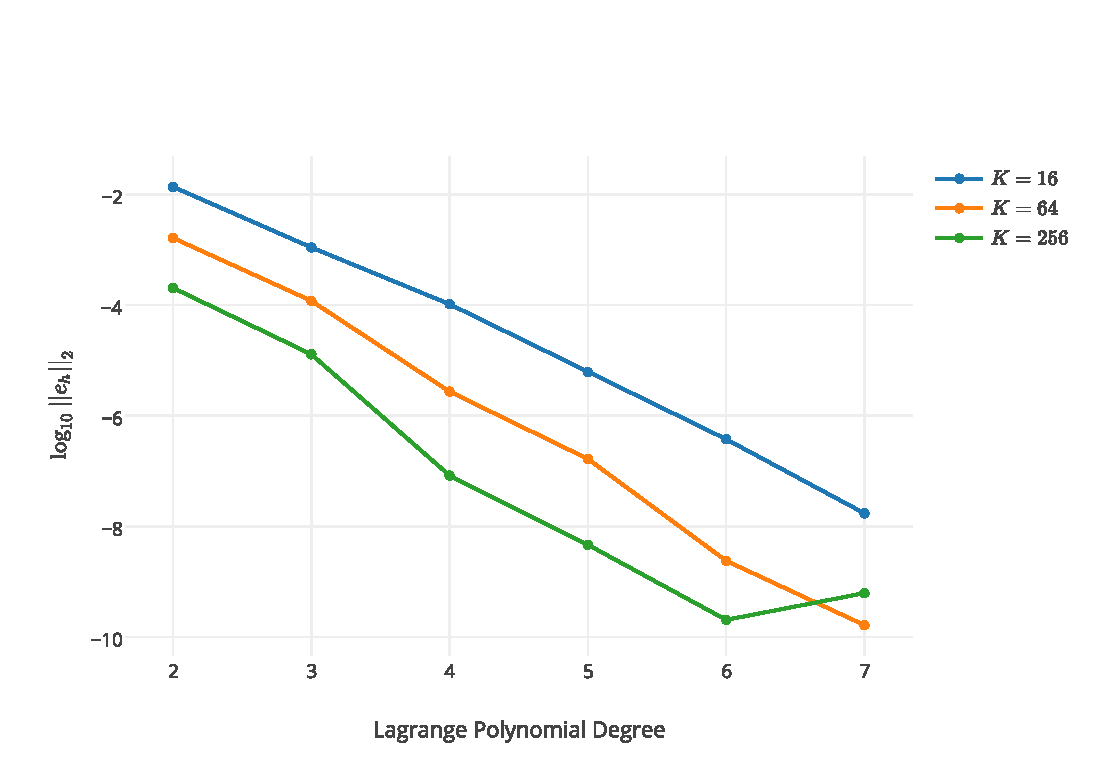
\includegraphics[width=\textwidth]{pictures/Kfixed.pdf}
% \end{mybox}     \\
% \vspace{.5cm}

  \end{column}
  \begin{column}{.48\textwidth}
{\tiny $\,\,\,$}\\
{\tiny $\,\,\,$}\\
{\tiny Below: Exponential and Algebraic convergence for a simple Poisson problem with h and p fixed respectively.}
% \vspace{.4cm}
% \begin{mybox}{white}{}
\vspace{-.3cm}
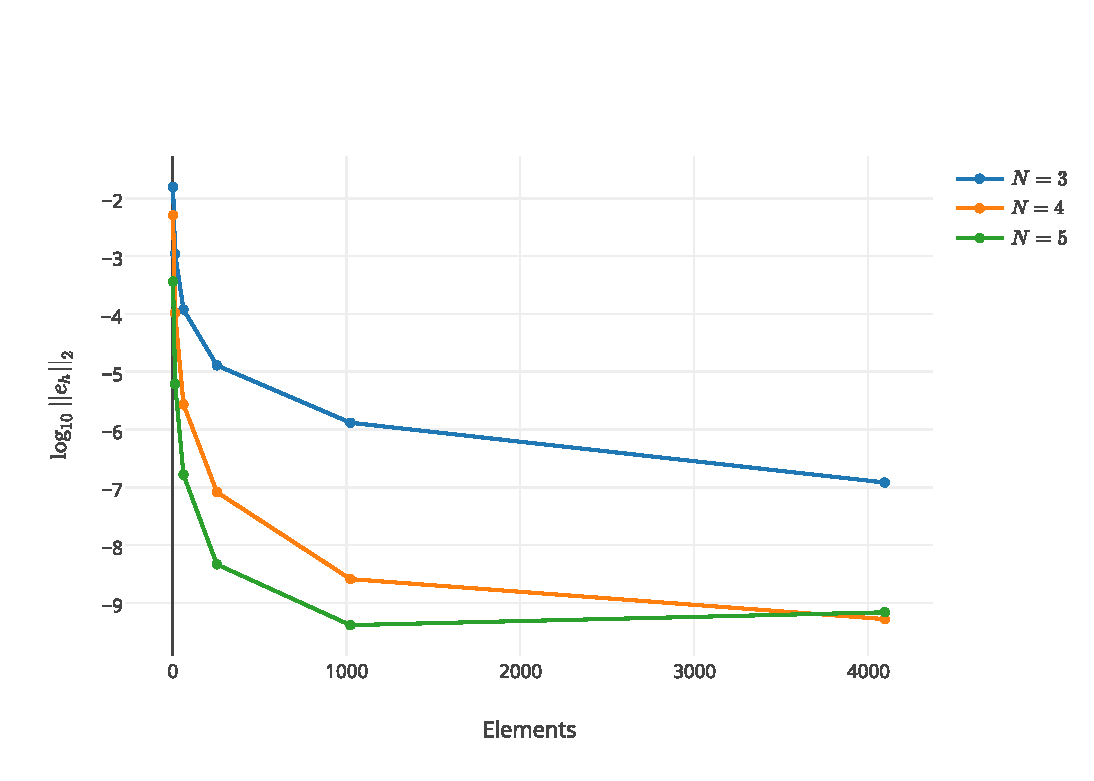
\includegraphics[width=\textwidth]{pictures/Nfixed.pdf}        
% \end{mybox}
  \end{column} 
\end{columns}


% \end{center}       
\end{mybox}

% and make incremental changes.





}

\subsection{Phase 1}

\frame{
  \frametitle{Phase 1.1: Puncture Initial Data}



\begin{columns}
  \begin{column}{.58\textwidth}
\scriptsize
\begin{mybox}{white}{\centering Multi-Black Hole Initial Data}
\begin{itemize}[leftmargin=*]
\item[\blacksquare]Each black hole is represented as a puncture in the manifold. 
\item[\blacksquare]3 of the 4 vacuum constraint equations are analytically solvable. 
\item[\blacksquare]Spins and momenta, $S^i$ and $P^{i}$ come in as free variables.
% \item[\blacksquare]Last remaining constraint equation:
\end{itemize}
\begin{equation*}
\label{eq:8}
-(\partial^2_x+\partial^2_y+\partial^2_z)u = \frac{1}{8}\Hat K^{ij} \Hat K_{ij} + 2\pi\rho\psi^{-3}. 
\end{equation*}
\end{mybox}
    \begin{mybox}{white}{\centering Estimated Time}
\centering {Mid-June to October 1st 2015}
\end{mybox}
  \end{column}
  \begin{column}{.4\textwidth}
    \begin{mybox}{white}{\centering \tiny Important Aspects of Stage}
\begin{itemize}[leftmargin=*]
\tiny
\item[\blacksquare]Can test scaling by placing third BH far away for BBH
\item[\blacksquare]nice test of hp-adaptivity \\($C^{4}$ smooth around punctures)
 \item[\blacksquare]scaling results/code debut in publication
\end{itemize}
% \hspace{-.5cm}
\end{mybox}
    \begin{mybox}{white}{\centering  \tiny Code Changes}
\tiny
\begin{itemize}[leftmargin=*]
\item[\blacksquare]add multigrid to 2-D code
\item[\blacksquare]convert to 3-D
\item[\blacksquare]add non-linear solver from PetSC
\item[\blacksquare]hp-adaptive mesh refinement
% \item[\blacksquare]three black-hole puncture initial data
% \item[\blacksquare]weak/strong scaling tests
% \item[\blacksquare]publication
\end{itemize}
\end{mybox}
  \end{column}
\end{columns}

}

\frame{
  \frametitle{Phase 1.2: TOV Initial Data in 3D}


\begin{columns}
  \begin{column}{.63\textwidth}
\scriptsize
\begin{mybox}{white}{\centering TOV Initial Data in 3D with EOS tables}
\begin{itemize}[leftmargin=*]
% \item[\blacksquare]Solve the TOV Initial-Data equations in 3-D. 
% \item[\blacksquare]Using a tabulated EOS 
\end{itemize}
\begin{equation*}
\label{eq:9}
\begin{split}
  &\frac{dp}{dr} = -G(\rho(1+\epsilon/c^{2}) + p/c^2) \frac{m + 4\pi r^{3} p/c^2}{r(r-2Gm/c^{2})}, \\
  &\frac{dm}{dr} = 4\pi r^2 \rho (1 + \epsilon/c^2), \\
  &\frac{d \ln(\alpha)}{dr} = \frac{m+4\pi r^{3}p/c^2}{r(r-2Gm/c^{2})}, \\
  &P = P(\rho) \,\,\,\,\,\, \text{(from table)}.
\end{split}
\end{equation*}
\end{mybox}
    \begin{mybox}{white}{\centering Estimated Time}
\centering October 1st to December 31st, 2015
\end{mybox}
  \end{column}
  \begin{column}{.4\textwidth}
    \begin{mybox}{white}{\centering \tiny Important Aspects of Stage}
\begin{itemize}[leftmargin=*]
\tiny
\item[\blacksquare]Tests hp-AMR against discontinuities with unknown location
\item[\blacksquare]Tests p4est on non-cubic domain
\item[\blacksquare]Required step for superimposed TOV initial-data
\end{itemize}
% \hspace{-.5cm}
\end{mybox}
    \begin{mybox}{white}{\centering  \tiny Code Changes}
\tiny
\begin{itemize}[leftmargin=*]
\item[\blacksquare] non-cubic domains
\item[\blacksquare] add yt visualization
% \item[\blacksquare]three black-hole puncture initial data
% \item[\blacksquare]weak/strong scaling tests
% \item[\blacksquare]publication
\end{itemize}
\end{mybox}
  \end{column}
\end{columns}
}


\subsection{Phase 2}

\frame{
  \frametitle{Phase 2: NS-\{NS,BH\} Initial-Data with Moderate C}

\begin{columns}
  \begin{column}{.58\textwidth}
\scriptsize
\centering
\begin{mybox}{white}{\centering \text{NS-\{NS,BH\}} + Moderate Compactness}
\begin{itemize}[leftmargin=*]
\item[\blacksquare]Solve the full Constraint Equations in 3D. 
\item[\blacksquare]Using a tabulated EOS with moderate compactness.
\end{itemize}
\end{mybox}
    \begin{mybox}{white}{\centering Estimated Time}
\centering January 1st to March 1st, 2016.
\end{mybox}
  \end{column}
  \begin{column}{.4\textwidth}
    \begin{mybox}{white}{\centering \scriptsize \tiny Important Aspects of Stage}
\begin{itemize}[leftmargin=*]
\scriptsize
\item[\blacksquare]can compare to SpEC results {\tiny [Henriksson et al; 2014]}
\item[\blacksquare]Publication detailing results
\end{itemize}
% \hspace{-.5cm}
\end{mybox}
%     \begin{mybox}{white}{\centering  \tiny Code Changes}
% \tiny
% \begin{itemize}
% \item[\blacksquare]add yt visualization
% % \item[\blacksquare]three black-hole puncture initial data
% % \item[\blacksquare]weak/strong scaling tests
% % \item[\blacksquare]publication
% \end{itemize}
% \end{mybox}
  \end{column}
\end{columns}

}


\subsection{Phase 3}

\frame{
  \frametitle{Phase 3: NS-\{NS,BH\} Initial-Data with High C}

\begin{columns}
  \begin{column}{.58\textwidth}
\scriptsize
\begin{mybox}{white}{\centering \text{NS-\{NS,BH\}} + High Compactness}
\begin{itemize}[leftmargin=*]
\item[\blacksquare]Solve the full Constraint Equations in 3D. 
\item[\blacksquare]Using tabulated EOSs and high compactness.
\item[\blacksquare]Extra schemes/constraints will have to be investigated in order to
get convergence
\end{itemize}
\end{mybox}
    \begin{mybox}{white}{\centering Estimated Time}
\centering June 1st, 2016 onwards.
\end{mybox}
  \end{column}
  \begin{column}{.4\textwidth}
    \begin{mybox}{white}{\centering \tiny Important Aspects of Stage}
\begin{itemize}[leftmargin=*]
\tiny
\item[\blacksquare]First ever initial-data in this regime
\item[\blacksquare]Publication detailing results
\end{itemize}
% \hspace{-.5cm}
\end{mybox}
%     \begin{mybox}{white}{\centering  \tiny Code Changes}
% \tiny
% \begin{itemize}
% \item[\blacksquare]add yt visualization
% % \item[\blacksquare]three black-hole puncture initial data
% % \item[\blacksquare]weak/strong scaling tests
% % \item[\blacksquare]publication
% \end{itemize}
% \end{mybox}
  \end{column}
\end{columns}

}


\subsection{Phase 4}

\frame{
  \frametitle{Phase 4: Other Simulations}

\begin{columns}
  \begin{column}{.58\textwidth}
\scriptsize
\begin{mybox}{white}{Newtonian Gravity Simulations}
\begin{itemize}[leftmargin=*]
\item[\blacksquare]With a powerful Elliptic Solver, other physics can be investigated. 
\item[\blacksquare]Newtonian gravity simulations (binary mergers with complex microphysics, galactic dynamics)
\end{itemize}
\end{mybox}
    \begin{mybox}{white}{\centering Estimated Time}
\centering Left-over/Unknown
\end{mybox}
  \end{column}
 %  \begin{column}{.4\textwidth}
%     \begin{mybox}{white}{\centering \tiny Important Aspects of Stage}
% \begin{itemize}
% \tiny
% \item[\blacksquare]First ever initial-data in this regime
% \item[\blacksquare]Publication detailing results
% \end{itemize}
% % \hspace{-.5cm}
% \end{mybox}
% %     \begin{mybox}{white}{\centering  \tiny Code Changes}
% % \tiny
% % \begin{itemize}
% % \item[\blacksquare]add yt visualization
% % % \item[\blacksquare]three black-hole puncture initial data
% % % \item[\blacksquare]weak/strong scaling tests
% % % \item[\blacksquare]publication
% % \end{itemize}
% % \end{mybox}
%   \end{column}
\end{columns}

}

\frame{

\frametitle{Questions?}

\begin{columns}
\begin{column}{.48\textwidth}
\begin{center}
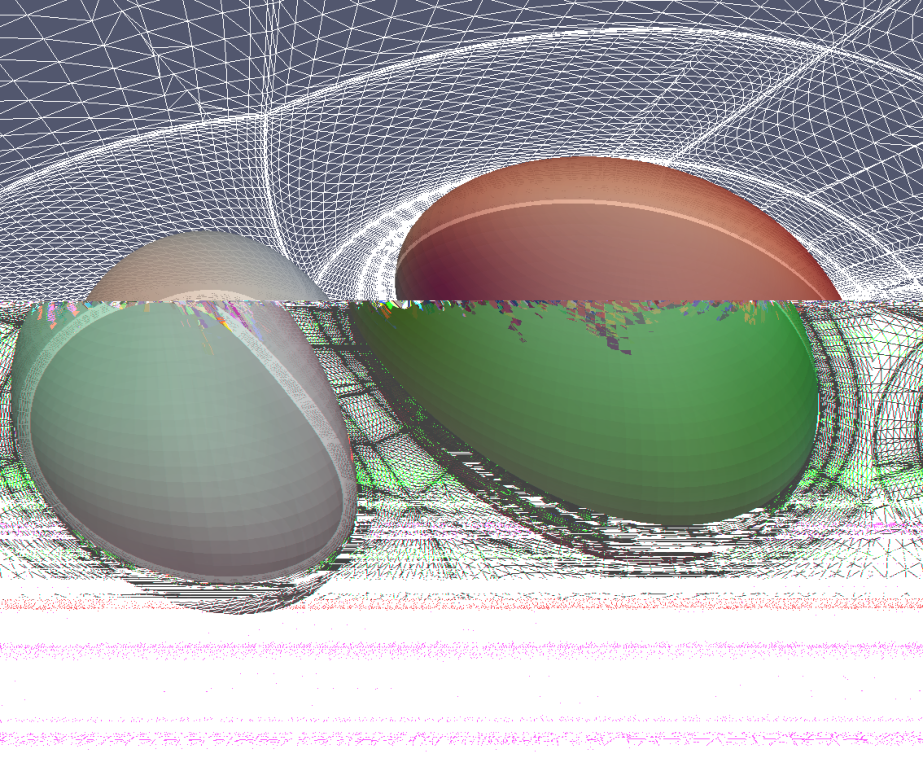
\includegraphics[width=.6\textwidth]{pictures/2bh.pdf}\\
\vspace{.1cm}
{\centering \tiny [BBH; Lovelace et al]}\\
\vspace{.2cm}
\includegraphics[width=.6\textwidth]{pictures/rezzolla.pdf}\\
\vspace{.2cm}
{\centering \tiny [NSNS; Rezzolla et al]}
\end{center}
\end{column}
\begin{column}{.48\textwidth}
\begin{center}
\includegraphics[width=.5\textwidth]{pictures/francois.pdf}\\
\vspace{.1cm}
{\centering \tiny [NSBH; Foucart et al]}\\
\vspace{.2cm}
\includegraphics[width=.5\textwidth]{pictures/ott.png}\\
% \vspace{.2cm}
{\centering \tiny [Supernova; Ott et al]}
\end{center}
\end{column}
\end{columns}

}

%%% Local Variables:
%%% mode: latex
%%% TeX-master: "main"
%%% End:
